\documentclass[../SWD_disp.tex]{subfiles}

\begin{document}
\section{GUI Design Patterns}
Hvorfor bruge et GUI pattern?

Det kan skabe bedre workflow i teams, nemmere at teste specielt nemmer for andre at dykke ned i, hvis det skal vedligeholdes.


\subsection{MVVM}
I forhold til MVC og MVP så er MVVM mere segregreret. Her prøves der nemlig skelne helt væk fra modellen.

\begin{figure}[H]
	\centering
	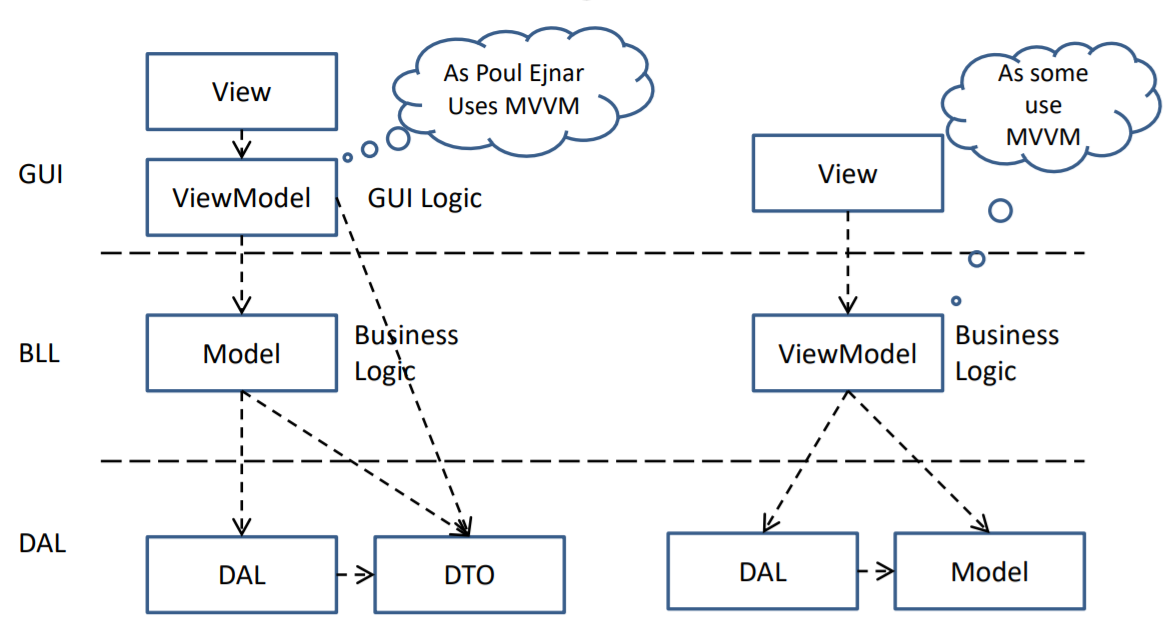
\includegraphics[width = 0.6\textwidth]{mvvm.png}
\end{figure}
\subsection{MVC + MVP}
Brugeren interagere med ``controlleren'' som ændre på modellen, som opdatere viewet. Set på billedet under.
\begin{figure}[H]
	\centering
	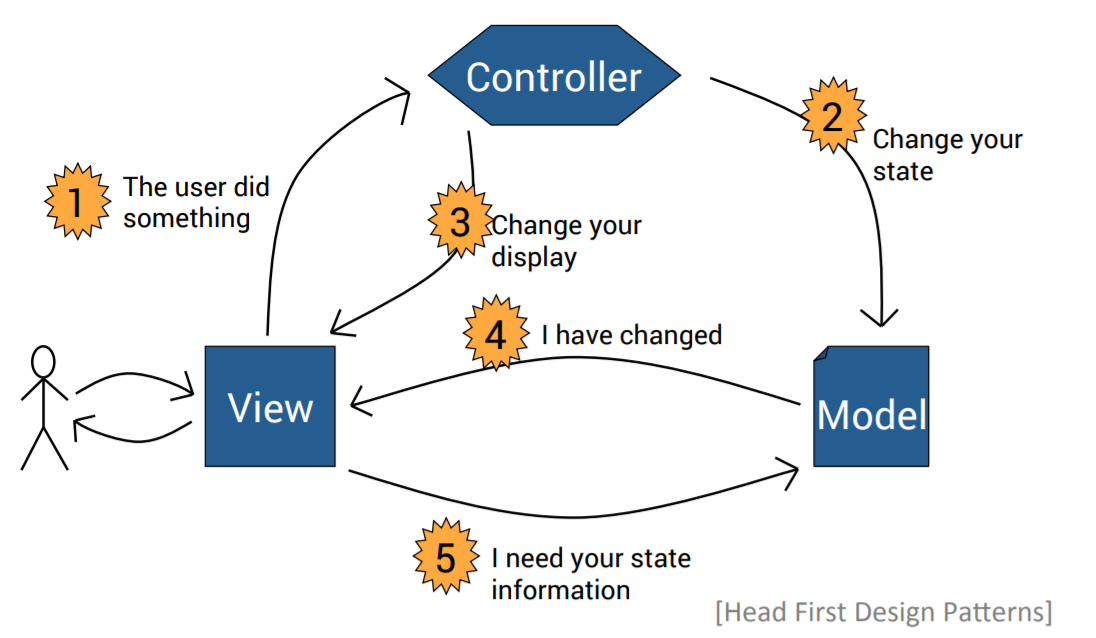
\includegraphics[width = 0.6\textwidth]{mvc.png}
\end{figure}
donger
\begin{enumerate}
	\item Superviser Controller
	\item Passive COntroller
\end{enumerate}
\end{document}
